\section{Theoreticals}
\subsection{Energy States of Rubidium and Zeemann-Effect}

According to rules of Quantum Mechanics, every atom has its own quantized energy states, in which the electrons are positioned. The states are described by some quantum numbers, which are called n, l and s. n is the energy quantum number, l describes the angular momentum and s shows the electron spin and obviously is $s=\frac{1}{2}$. We notate these states as 1S, 2S, 2P and so on.
The angular momentum and spin couple to the so-called finestructur. This are some energy corrections to the states, which also can split up through this coupling. Mathematically, we add the quantum numbers l and s to the total angular momentum j. Because the directions of l and s can be the same or different, we get in the case of l=1 two different possibilities for J, which are generated by $J=\frac{1}{2}$ and $J=\frac{3}{2}$ and have different energy niveaus. Our notations changes so to $1S_{\frac{1}{2}}, 2S_{\frac{1}{2}}, 2P_{\frac{1}{2}}, ...$.

For the complete correct energy niveaus, we have to add another quantum number, which describes the spin of the atomcore. It is called I and counts $I=\frac{3}{2}$ in our case, as we work with $^{87}Rubidium$. The angular momentum I therefore adds to the total angular momentum J to another total angular momentum called F. The resulting energy states are called hyperfinestructur.

In Figure \ref{states} are plotted the S and P states of Rb. Addiotionally there are marked the wavelenghts  for the energy difference of the different states and the magnetic quantum number m, which always appear with an angular momentum quantum number. In our case, the resulting angular momentum quantum number is F and $m_f$ always runs from -F to F, so the figure can be understood well. Without external fields, the energy of all states with different values of m is exactly the same, so usually there is no such splitting seen.

\begin{figure}[htbp] 
     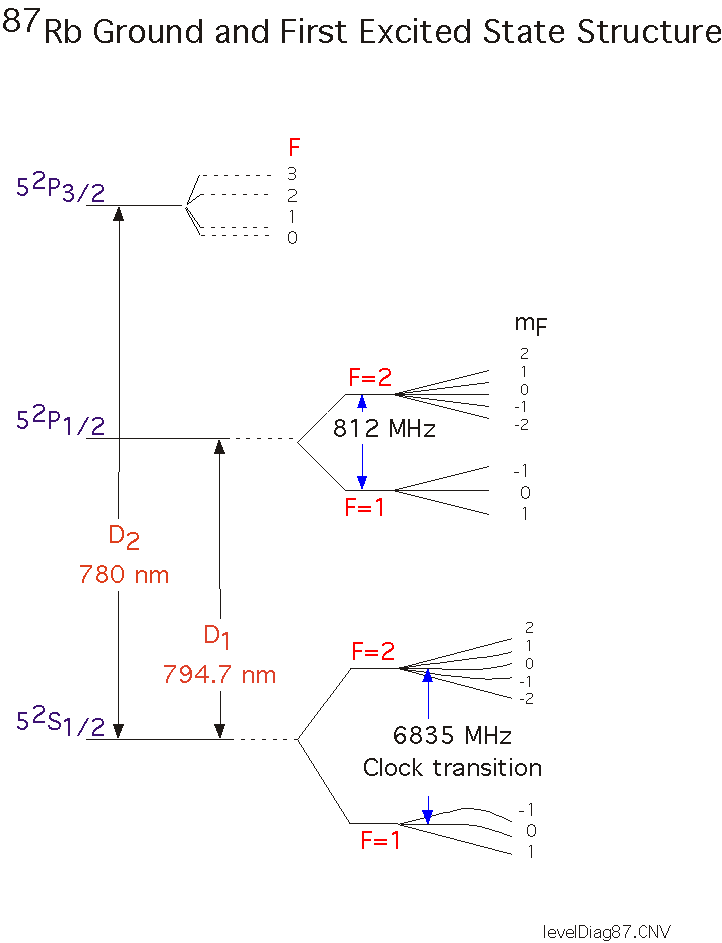
\includegraphics[scale=0.7]{level87.png}
  \caption{Energy states of $^{87}Rb$}
  \label{states}
\end{figure}

The existence of these magnetic quantum numbers is responsible for the so-called zeeman-effect, which appears if we put our atom in a small magnetic field. It is possible to calculate the energy correction effect of the magnetic coupling of external field and orbital angular momentum. The correction counts $E_Z=g_F\mu_0 Bm_f$
According to that, we now have different energx levels for different values of $m_f$. Our old energy states is so split up in $2F+1$ states with different energies, which are separated by the same energy difference. $g_F$ is the Landé-factor, which is different in every state of the hyperfinestrucutr can be calculated by:

\begin{align}
g_F=g_J \frac{F\left(F+1\right)+J\left(J+1\right)-I\left(I+1\right)}{2F\left(F+1\right)}
\end{align}

And continued:

\begin{align}
g_J=1 + \frac{J\left(J+1\right)+S\left(S+1\right)-L\left(L+1\right)}{2J\left(J+1\right)}
\end{align}

\subsection{Optical Pumping}
If there is light of a certain wavelenght ($794.7nm$), the electrons in the Rubidium atom can be raised from the groundstate $^2S_{1/2}$ to the first excited state $^2P_1/2$. But for this transition there is a transition rule that has to be followed. A circularly polarized photon has an angular momentum of an amount of $1\hbar$. We will call the light $\sigma^+$ if the photons have a positive angular momentum relative to the direction of the applied magnetic field. Similarly we call the light $\sigma^-$ if the photons have a negative angular momentum relative to the magnetic field. As an example right-polarized light parallel to the magnetic field would be $\sigma^+$. At last linearly polarized light is called $\pi$ and does not have an angular momentum.

Now you can look at the absorbtion af an $\sigma^+$-photon in the Rubidium 87 gas. The photon vanishes and for the conservation of angular momentum the angular momentum of the electron has to increase by 1. This means to the quantum number $m_f$ has to be added 1, if it is possible. There do not exist states with $m_f=+3$, so the atoms in the $+2$ state do not absorb $\sigma^+$-photons. For $\sigma^-$ $m_f$ decreases by 1 and $\pi$ doesn't change the quantum number $m_f$. Due to spontaneous radiation emission the atoms can return to the groundstate. Within this process they are emitting $\pi, \sigma^+$ or $\sigma^-$ photons so that all groundstate sublevels can be populated again.

Now we only have $\sigma^+$ pumping light and because of the continual absorbtion and emission the quantum numbers $m_f$ of the atoms will be raised gradually until they reach $+2$. There the atoms are trapped and a nonthermal distribution is acheived. Processes where a nonthermal ditribution is acheived by light is called optical pumping in general.

When the maximum population of $m_f=+2$ is reached the excitation of the atoms by the $\sigma^+$ photons is at minimum and so the Rubidium gas becomes the most transparent for the light. The intensity after the light has passed the gas can be used to measure the degree of polarization of the gas. There are always some radiative transitions to the groundsate, but this doesn't compensate the absorbtion. Additionally there can be nonradiative transitions as an efect of collisions which also lead the atoms in the ground state. So even  when the gas has reached its most transparent phase, the gas still absorbs some light.

\subsection{Stimulated emission}
As we learned in the pervious section, we can raise electrons to an upper energy state by light with a certain wayelength. If all electrons are raised in the upper energy state with $m_f=2$ and we continue to radiate light with wavelenght of the energy difference of the states, we can also get another effect called stimulated emission. Thereby, the incoming photon is not absorbed, but induces another photon with the same wavelength, which is emitted. The electron then loses energy and is dropped back to the old lower energy state. The two or more photons are coherent and have exactly the same wavelength, so the built radioation can be used for example to build a laser. This effect can also be reached by an alternating magnetic field, which oscillates with the frequency of $\nu=g_F \frac{e}{4\pi m_f}B$.





